% vim: spell spelllang=en_us
\documentclass[conference,11pt]{IEEEtran}
\usepackage[T1]{fontenc}
\usepackage[utf8]{inputenc}
\usepackage[english]{babel}
\usepackage{csquotes}
\usepackage{biblatex}
\usepackage{amsmath}
\usepackage{amsthm}
\usepackage{amssymb}
\usepackage{minted}
\usepackage{tipa}
\usepackage{mdframed}
\usepackage[inline]{enumitem}

\addbibresource{../references.bib}

\MakeOuterQuote{"}
\setminted{autogobble,python3,mathescape,frame=lines,framesep=2mm,fontsize=\footnotesize}

\usepackage{pgfplots}
\pgfplotsset{compat=newest}

\newtheorem{definition}{Definition}

\title{Applications and Implementation of Differential Privacy on Statistical
Databases}
\author{%
    \IEEEauthorblockN{%
        Jonathan Sumner Evans\IEEEauthorrefmark{1},
        Victoria Girkins\IEEEauthorrefmark{2}, and
        Sam Sartor\IEEEauthorrefmark{3}
    }
    \IEEEauthorblockA{%
        Department of Computer Science,
        Colorado School of Mines\\
        Golden, Colorado\\
        Email:
            \IEEEauthorrefmark{1}jonathanevans@mines.edu,
            \IEEEauthorrefmark{2}vgirkins@mines.edu,
            \IEEEauthorrefmark{3}ssartor@mines.edu,
    }
}

\begin{document}

\maketitle

% (1) an abstract
\begin{abstract}
    Statistical databases have long been know to be vulnerable to inference
    attacks.  We describe the nature of inference attacks and analyze one method
    of mitigating these attacks called Differential Privacy. We discuss two
    mechanisms for differential privacy. We then explain our implementation of a
    simple Differential Privacy statistical database and the experiments we
    performed on the database. We then analyze how well our implementation
    achieves the objectives of Differential Privacy databases. We conclude by
    calling on industry to create differential privacy implementations that can
    be used in general applications.
\end{abstract}

% (2) introduction (including the background, motivation, and goal)
\section{Introduction}
Statistical databases are designed for statistical analysis of the datasets
contained within the database. One of the desired properties of statistical
databases is that nothing about an individual should be learnable from the
database that cannot be learned without access to the
database~\cite{Dwork:2006:DP}. In other words, gathering information about the
records underlying the statistics using allowed queries on the database should
be impossible.

Without any protections, well-crafted queries to a statistical database can
implicitly reveal private information.  This attack is know as an
\textit{inference attack}.  To prevent these attacks, the key case to consider
is that of two databases which differ by only a single row.  Consider, for
example, a database which associates people with their incomes.  The query

\begin{minted}{sql}
    SELECT SUM(income) FROM table
\end{minted}
seems harmless at first. But if a new record were added and we ran the query
again, the difference between the two results represents the exact income of the
new entry. If the attacker knows the identity of the person who was added, the
privacy leak becomes even more severe.

Of course, an attacker may not have the luxury of always knowing when a new
record will be added to the database, and of timing his queries accordingly. He
may, however, achieve the same results by narrowing down his query with
conditionals.

\begin{minted}{sql}
    SELECT SUM(income)
      FROM table
     WHERE zip != 80127
\end{minted}
may be sufficient in a small enough database, or more conditionals may need to
be added to ensure the queries jointly isolate a single row. However, since the
danger occurs when information about a single entry is returned, regardless of
how the attacker managed it, we will assume for simplicity's sake that the
database is queried before and after the addition of a single row.

\subsection{Previous Attempts at Anonymizing Statistical Data}
Many attempts have been made to privatize data in the past and many are still in
use today. However everything from simply removing columns containing personally
identifiable information to advanced techniques such as as k-anonymity and
l-diversity have been shown to be vulnerable to attack~\cite{Atockar:2014}.
K-anonymity, for example, does not include any randomization, attackers can
still make inferences about data sets~\cite{Aggarwal:2005}.

\subsection{Differential Privacy}
In 2006, Cynthia Dwork proposed a new technique to reduce the risk of a
successful inference attack called \textit{Differential
    Privacy}~\cite{Hilton:DP:history}. The goal of Differential Privacy is to
maximize the statistical accuracy of queries on a statistical database while
also maximizing the privacy of the individual records. It does this by
introducing noise into the dataset. This randomness reduces the likelihood of
obtaining meaningful information about the individual records in the database.

The real power of Differential Privacy is when it is used in conjunction with a
privacy bound, $\varepsilon$ as described in Section~\ref{sec:epsilon-dp}. The
methods for generating random noise are discussed in Section~\ref{sec:dp-mech}.
Details about how the one of the mechanisms is used to ensure differential
privacy are explained in Section~\ref{sec:using-laplace-dp}.

\subsubsection{Epsilon-Differentially Private}\label{sec:epsilon-dp}
One useful way of discussing Differential Privacy is to talk about what it means
for a database to be \textit{epsilon-differentially private}. A database falls
under this category if it is private as bounded by a chosen value epsilon. As
opposed to the mathematical definition, here we give a more intuitive definition
as stated by Atockar~\cite{Atockar:2014}:

\blockquote{%
    This [epsilon-differentially private] can be translated as meaning that the
    risk to one's privacy should not substantially (as bounded by epsilon)
    increase as a result of participating in a statistical database.
}

For the sake of rigorousness, the formal mathematical definition of
epsilon-differential privacy described by Dwork~\cite{Dwork:2006:DP} follows.

\begin{mdframed}
    \begin{definition}
        A randomized function $\mathcal{K}$ gives
        \textbf{\textepsilon-differential privacy} if for all data sets $D$ and
        $D'$ differing on at most one row, and all $S \subseteq
        Range(\mathcal{K})$,
        \begin{equation}
            \Pr[\mathcal{K}(D) \in S] \leq \exp(\varepsilon) \times
            \Pr[\mathcal{K}(D') \in S]
        \end{equation}
    \end{definition}
\end{mdframed}

For now, all that concerns us about this equation is that $D$ and $D'$ are the
above-mentioned databases differing by a single row, and $\mathcal{K}$ is our
mechanism for adding noise drawn from our distribution as described in
Section~\ref{sec:dp-mech}.

\subsubsection{Differential Privacy Mechanisms}\label{sec:dp-mech}
There are two primary Differential Privacy Mechanisms: the Exponential Mechanism
and the Laplace Mechanism. The Exponential Mechanism should be used on
categorical, non-numeric data. For example queries of the form ``what is the
most common eye color in this room'' should be protected using the Exponential
Mechanism~\cite{Atockar:2014}. The Laplace Mechanism should be used with
non-categorical, real-value data~\cite{Geng:2014}. Because of the nature of our
data, our primary focus for this project is the Laplace Mechanism.

Before we rigorously examine the mathematics, let us review our inputs and our
goals:

\begin{itemize}[leftmargin=4em]
    \item [\textbf{Inputs}] A statistical database with sensitive information,
        an attacker poised with a malicious query, and a desired epsilon, or
        privacy parameter.

    \item [\textbf{Goals}] To add enough Laplace-distributed noise to the
        results of database queries that our database is mathematically
        considered differentially private.
\end{itemize}

% make Definition of Laplace Distribution not break across columns
{\vfill\eject}

% Have to include this table here so it shows up on the next page
\begin{table*}[h]
    \caption{Columns in Our Sample Dataset}
    \label{tab:cols}
    \centering
    \begin{tabular}{l | l | l}
        \textbf{Field} & \textbf{Column Name} & \textbf{Method of Generation} \\
        \hline
        Name & \texttt{name} & the \texttt{names} Python library \\
        Age & \texttt{age} & uniformly distributed between 18 and 65 \\
        Income & \texttt{income} & distributed log-normal \\
        Zip Code & \texttt{zip} & from a random set of \textasciitilde40
            five-digit numbers \\
        Net-worth & \texttt{net\_worth} & from age, income, and a random offset
    \end{tabular}
\end{table*}

Mathematically, the Laplace Distribution is defined as follows:
\begin{mdframed}
    \begin{definition}
        The Laplace Distribution, $\text{Lap}(\mu, b)$, also known as a
        symmetric exponential distribution, is the probability distribution with
        p.d.f.:
        \begin{equation}
            P(x|\mu, b) = \frac{1}{2b}\exp\left(-\frac{|x - \mu|}{b}\right)
        \end{equation}
        where $\mu$ is the location of the center of the distribution and $b$ is
        the scale parameter.

        Figure~\ref{fig:laplace-pdf} is a visualization of the p.d.f.\ for a few
        values of $\mu$ and $b$.\\

        \begin{figure}[H]
            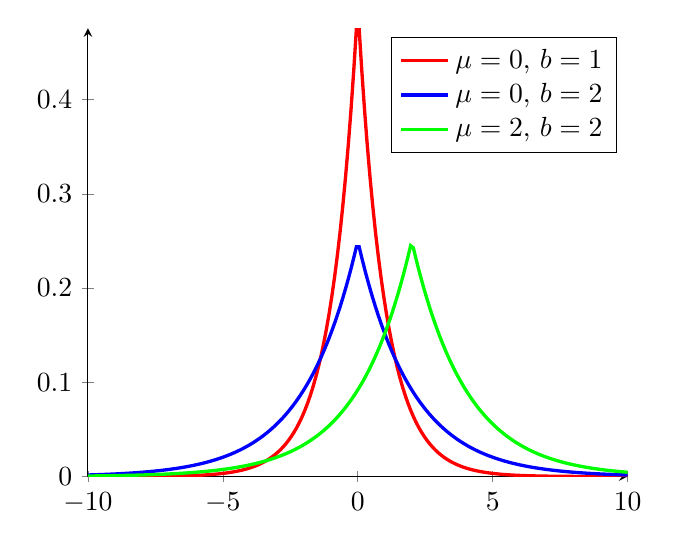
\begin{tikzpicture}
                \begin{axis}[axis lines = left]
                    \addplot [domain=-10:10, samples=200, color=red, very thick]
                    {(1 / 2) * exp(-abs(x))};
                    \addlegendentry{$\mu=0$, $b=1$}
                    \addplot [domain=-10:10, samples=200, color=blue, very thick]
                    {(1 / (2 * 2)) * exp(-abs(x) / 2)};
                    \addlegendentry{$\mu=0$, $b=2$}
                    \addplot [domain=-10:10, samples=200, color=green, very thick]
                    {(1 / (2 * 2)) * exp(-abs(x - 2) / 2)};
                    \addlegendentry{$\mu=2$, $b=2$}
                \end{axis}
            \end{tikzpicture}
            \caption{Probability Density Function for the Laplace Distribution}
            \label{fig:laplace-pdf}
        \end{figure}
    \end{definition}
\end{mdframed}

For us, $\mu$ is 0 so we can use a variant of the Laplace Distribution called
the Zero-Centered Laplace Distribution which has only one parameter, $b$, the
scale.

\subsubsection{Using the Laplace Differential Privacy Mechanism}\label{sec:using-laplace-dp}
In choosing the value for $b$, it makes sense that we should consider
\textepsilon, which quantifies the level of privacy we desire. Another factor
comes into play, however: the "sensitivity" of the database. This is defined as
the maximum difference between the results of any query run on two databases
which differ by only one row, as described above~\cite{Atockar:2014}. We shall
assume

\begin{minted}{sql}
    SELECT SUM(income) FROM table
\end{minted}
is the only query that this database will accept, so the "sensitivity" of our
database is clearly the highest income in the table, since this value will be
the difference between two queries run on the database before and after the
record associated with this income is added.

So, we must add noise while considering both {\textepsilon} and the database's
above-defined sensitivity. In fact, in a paper by
Dwork~\cite{Dwork:2011:private-data-analysis}, it was proven that choosing the
"scale" parameter ($b$) of our Laplace distribution according to this equation
\begin{equation}
    b = {\Delta}f/\varepsilon
\end{equation}
where ${\Delta}f$ is sensitivity, our database will mathematically satisfy
epsilon-differential privacy. That is, we should add noise to the data drawn
from a 0-centered Laplace distribution with scale parameter
${\Delta}f/\varepsilon$.

The one further consideration we must make is the possibility of multiple
queries to the database. The Laplace distribution is symmetrical, so if
unlimited queries were allowed, the attacker could simply run his query many
times and take the average to extract sensitive data. So we must limit the
number of queries allowed, and fortunately the calculation is linear. Assume we
draw all noise from the same distribution (it would be possible to vary it but
this unnecessarily complicates things), and that this distribution is Laplace,
0-centered, with a privacy parameter $\varepsilon_i$ (that is, with scale
parameter ${\Delta}f/\varepsilon_i$). If we limit learners to $k$ queries, our
overall privacy budget is $k\varepsilon_i$. This privacy budget is our
actual epsilon; as stated by Atockar, "it reflects the maximum privacy release
allowable for the total query session"~\cite{Atockar:2014}.

So to sum it up practically: if we wish to make our database
epsilon-differentially private as bounded by some value epsilon, our database
has sensitivity ${\Delta}f$, and we wish for learners to be allowed $k$ queries
before being locked out, we should add a random variable to each query, drawn
from the 0-centered Laplace distribution with scale parameter $k \times
{\Delta}f/\varepsilon$.

Of course, the lower of a privacy budget we allow, the noisier the data returned
by the queries will become~\cite{Atockar:2014}. If our queries become useless
due to the noise in the data, we may choose to raise the privacy budget---that
is, to increase the value of epsilon---or to further limit the number of queries
each user is allowed---that is, to lower the value of $k$. As with many issues
in information security, this is a balancing act between security and usability,
and we should consider the nature of the database, its contents, and its purpose
when choosing where to draw this line.

\begin{center}***\end{center}

For our final project, we implemented and analyzed a differential privacy
database which can perform a limited set of aggregate functions on a dataset.
We describe our approach and experiment in Section~\ref{sec:approach}. The
results of our experiment are summarized in Section~\ref{sec:results} and we
discuss some of the limitations of our implementation in
Section~\ref{sec:limitations}. In Section~\ref{sec:future-work} we describe some
of the potential future work in the field of differential privacy. We conclude
in Section~\ref{sec:conclusion} and call on industry to create effective,
easy-to-use differential privacy implementations for inclusion in general
industry applications.

% (3) key idea and approach (e.g., survey, testbed, system
% design/implementation, experiments, etc.)
% (4) activities (such as literature study and experiments) that you performed
\section{Approach and Experiment}\label{sec:approach}
To perform our experiment, we generated a large sample dataset suitable for
statistical queries (Section~\ref{sec:dataset}). Then we built a simple
Differential Privacy database as detailed in Section~\ref{sec:db-impl} and
crafted a set of queries with which to attack our database as described in
Section~\ref{sec:crafted-queries}.
% TODO: more here?

\subsection{Dataset}\label{sec:dataset}
To test our database, we created a dataset with 10,000 data points (rows). The
columns for each row are listed in Table~\ref{tab:cols}.

We chose the generation methods to roughly model the distributions of names,
age, income, zip code, and net worth of the US population. For example, the
income is distributed log-normal which approximates the distribution of incomes
in the United States.
% TODO: more here

\subsection{Database Implementation}\label{sec:db-impl}
% TODO: reads CSV
% TODO: implemented sum, count, min, max, mean, variance, sd
% TODO:         How to compute statistic (e.g. mean = total / count)
% TODO          How to find Δf (e.g. from most extreme value) 
% TODO: Filters rows with user-specified where clause (python expression)
% TODO: Handles edge cases where 1 or 0 rows are returned
% TODO: Adds laplace noise dependent on Δf, and a given ε / query limit
% TODO: Displays the privatized result
% TODO: more here

\subsection{Crafted Queries}\label{sec:crafted-queries}
% TODO: more here

% (5) description and analysis of the key results and observations
\section{Results}\label{sec:results}
% TODO: more here

% (6) discussion of the limitations and potential future work
\section{Limitations}\label{sec:limitations}
Our differential privacy implementation is very limited. Some of the limitations
are listed below.
\begin{itemize}
    \item Our implementation does not parse actual SQL queries. However, we
        have designed our program in a way that makes it easy to add a parsing
        engine on top of our program.
    \item Our implementation only works on a small set of aggregate functions.
        Future iterations of this project could implement more of these
        functions.
    \item Our implementation supports a very limited set of SQL operations. For
        example, it does not support \texttt{join} statements.  Future
        iterations of this project could implement more of the SQL standard.
    \item Our implementation can only process numerical data and is limited to
        the Laplace Mechanism. Adding alternative differential privacy mechanism
        such as the Exponential Mechanism would greatly improve the practicality
        of our differential privacy implementation.
    \item Our implementation is not heavily optimized. Currently, each query has
        $\mathcal{O}(n^2)$ algorithmic complexity. In further iterations of our
        implementation, we could improve the performance of our system using
        caching methods and by optimizing the algorithms we are using.
\end{itemize}

Although our differential privacy implementation is limited, it was very
effective for our experiment.
% TODO: add more here?

\section{Future Work}\label{sec:future-work}
Differential Privacy is a relatively new method of protecting data in a
statistical database. As such, there are not many implementations of it outside
of academia and large companies like Microsoft and Apple. If differential
privacy was adopted by a larger percentage of the industry, more statistical
databases with sensitive information would be resistant to inference attacks.

Software engineers have a great opportunity to create implementations of
differential privacy suitable for use in general industry applications. Such an
implementation could be a library which other programmers could include in their
project using dependency managers such as \texttt{pip}, \texttt{npm}, or
\texttt{cargo}. The creation of these general-purpose libraries could help make
differential privacy more accessible and cost effective for industry
professionals. This would help increase adoption of differential privacy and
result in an overall improvement of user's privacy in the industry.
% TODO: more here?

% (7) conclusion
\section{Conclusion}\label{sec:conclusion}
% What we expected
% What we got
% Limitations of our work
% Limitations of DP
% call on industry to make DP libraries
% TODO: more here?

% (8) references
{\printbibliography}

\end{document}
